\section{Hiện thực trò chơi}
\subsection{Gameplay chủ đạo}
Sau đây là một số hình minh họa về cơ chế chiến đấu chủ đạo của trò chơi.
\begin{figure}[H]
	\centering
	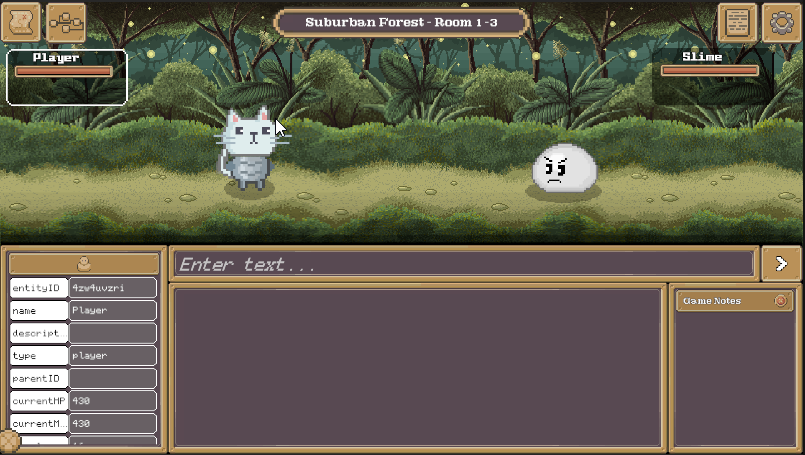
\includegraphics[width=13cm]{Images/gameplay1.png}
	\vspace{0.5cm}
	\caption{}
\end{figure}

\begin{figure}[H]
	\centering
	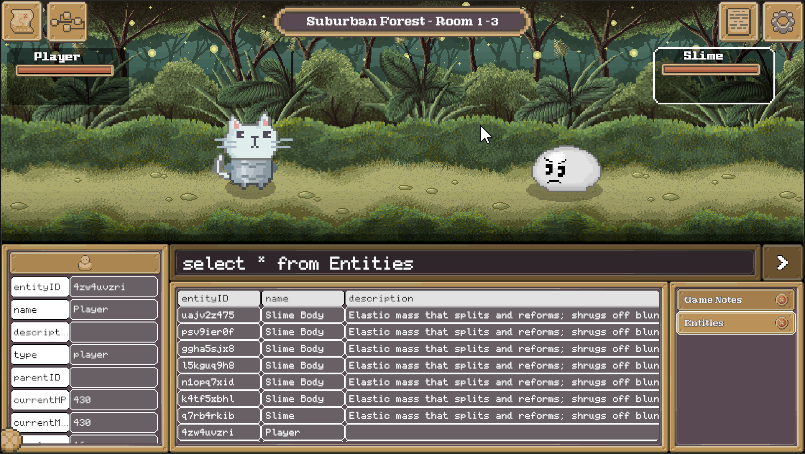
\includegraphics[width=13cm]{Images/gameplay2.png}
	\vspace{0.5cm}
	\caption{}
\end{figure}

\begin{figure}[H]
	\centering
	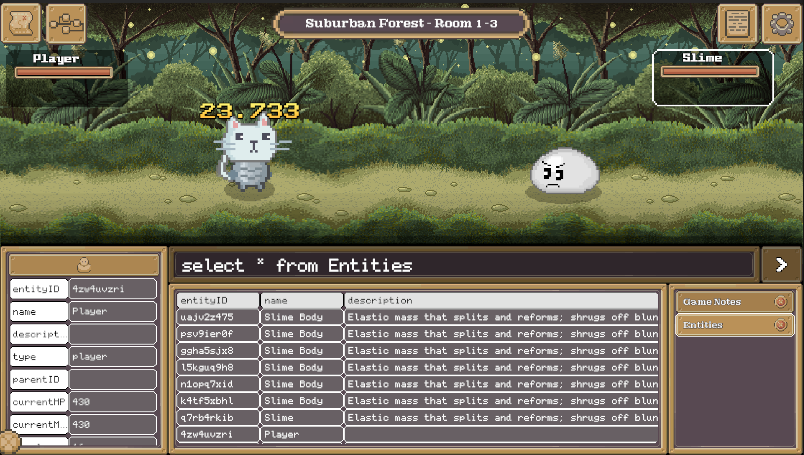
\includegraphics[width=13cm]{Images/gameplay3.png}
	\vspace{0.5cm}
	\caption{}
\end{figure}

\begin{figure}[H]
	\centering
	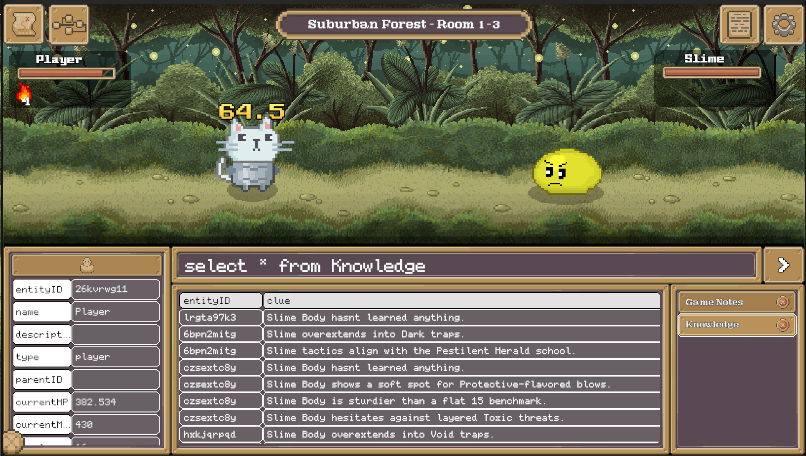
\includegraphics[width=13cm]{Images/gameplay4.png}
	\vspace{0.5cm}
	\caption{}
\end{figure}

\begin{figure}[H]
	\centering
	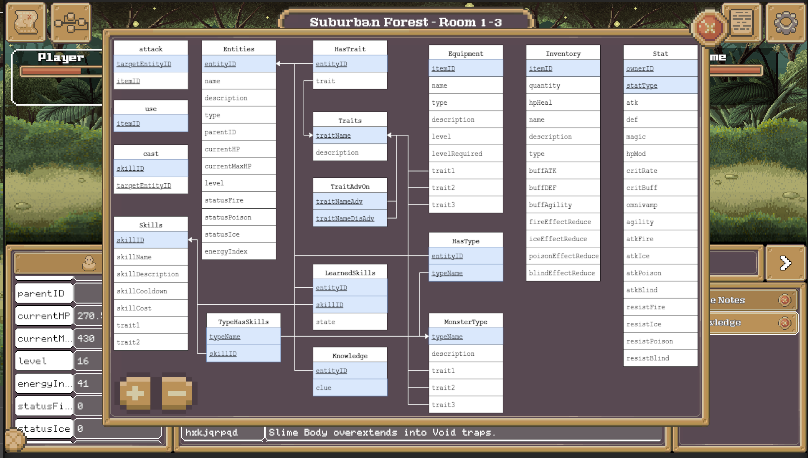
\includegraphics[width=13cm]{Images/gameplay5.png}
	\vspace{0.5cm}
	\caption{}
\end{figure}

\begin{figure}[H]
	\centering
	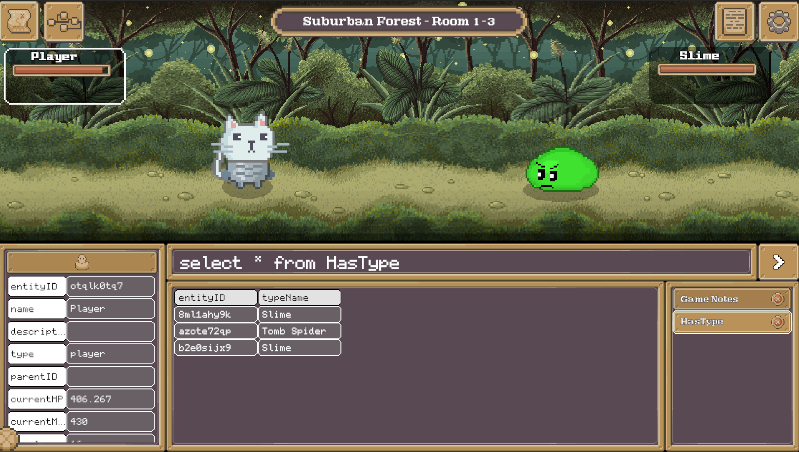
\includegraphics[width=13cm]{Images/gameplay6.png}
	\vspace{0.5cm}
	\caption{}
\end{figure}

\begin{figure}[H]
	\centering
	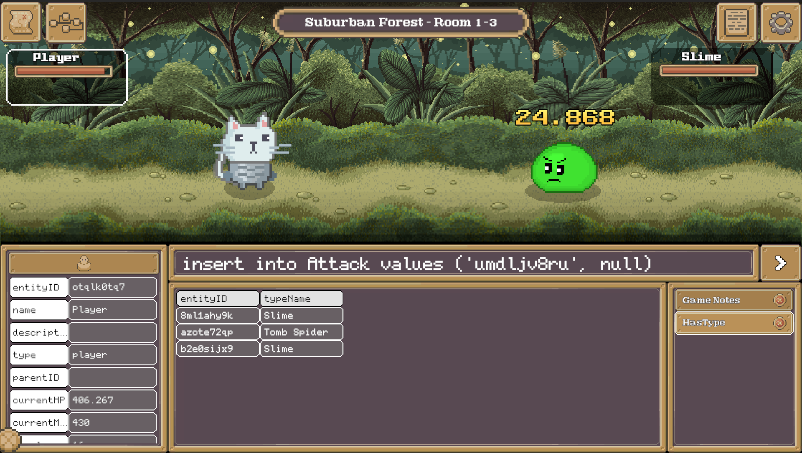
\includegraphics[width=13cm]{Images/gameplay7.png}
	\vspace{0.5cm}
	\caption{}
\end{figure}

\begin{figure}[H]
	\centering
	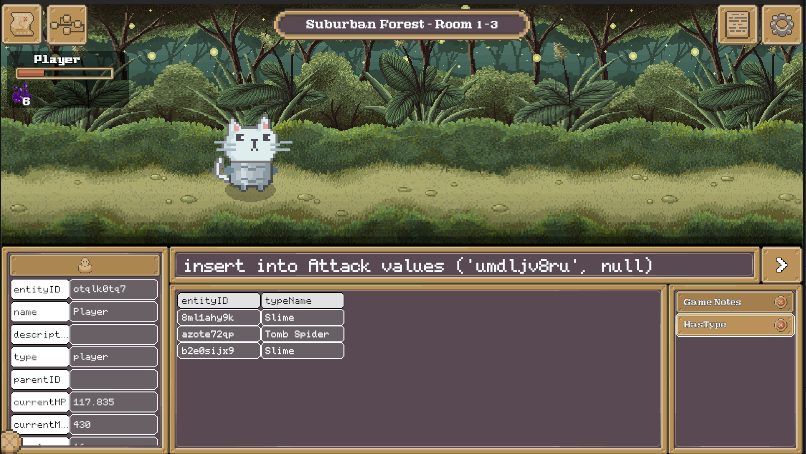
\includegraphics[width=13cm]{Images/gameplay8.png}
	\vspace{0.5cm}
	\caption{}
\end{figure}


\subsection{UI trong màn chơi}
Phần lớn các UI trong trò chơi đều được kế thừa từ class CanvasBaseView nhằm tái sử dụng những chức năng cơ bản như: hiện, ẩn hoặc toggle giữa 2 trạng thái.
\begin{figure}[H]
	\centering
	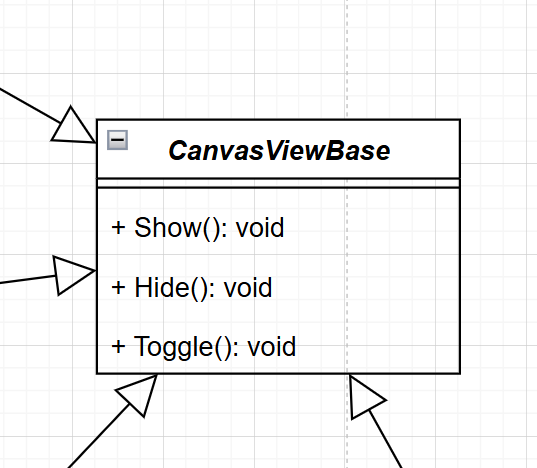
\includegraphics[width=7cm]{Images/CanvasViewBase.png}
	\vspace{0.5cm}
	\caption{CanvasViewBase}
\end{figure}

\subsubsection{UI tham khảo schema diagram}

Người chơi có thể mở một tab để tham khảo schema diagram của trò chơi và phóng to thu nhỏ tùy ý để tiện quan sát. Từ đó lập những chiến lược hợp lý để đánh bại quái vật và vượt qua màn chơi.

\begin{figure}[H]
	\centering
	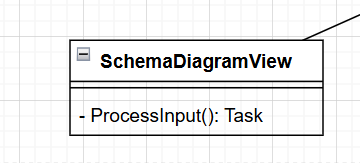
\includegraphics[width=7cm]{Images/SchemaDiagramView.png}
	\vspace{0.5cm}
	\caption{Schema diagram view}
\end{figure}

\begin{figure}[H]
	\centering
	\includegraphics[width=13cm]{Images/SchemaDiagramUi.png}
	\vspace{0.5cm}
	\caption{Minh họa UI Schema diagram view}
\end{figure}

\subsubsection{UI tham khảo cú pháp SQL cơ bản}

Cửa sổ tài liệu giúp người chơi tra cứu những câu lệnh SQl cơ bản được giải thích và đưa ra ví dụ minh họa.

\begin{figure}[H]
	\centering
	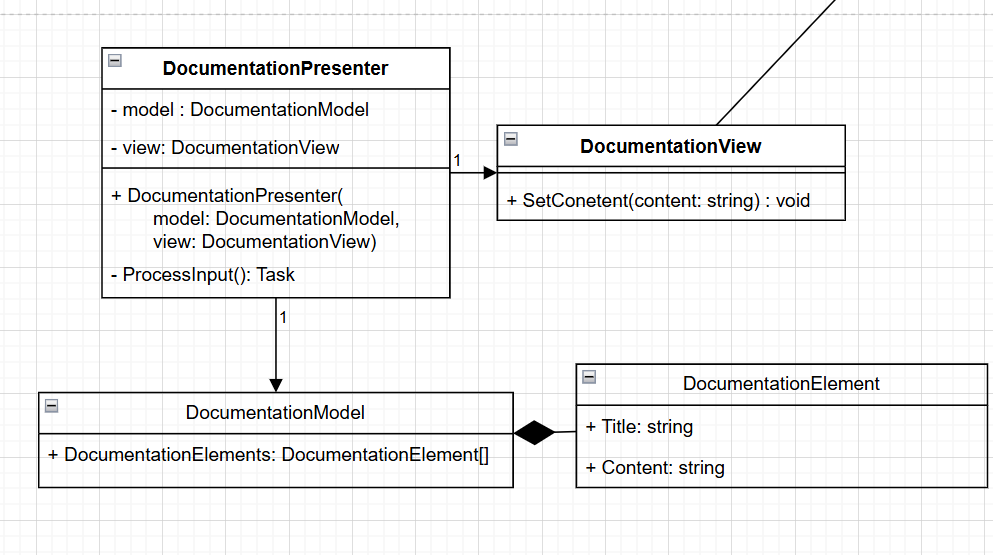
\includegraphics[width=13cm]{Images/DocumentationView.png}
	\vspace{0.5cm}
	\caption{Documentation class diagram}
\end{figure}

\begin{figure}[H]
	\centering
	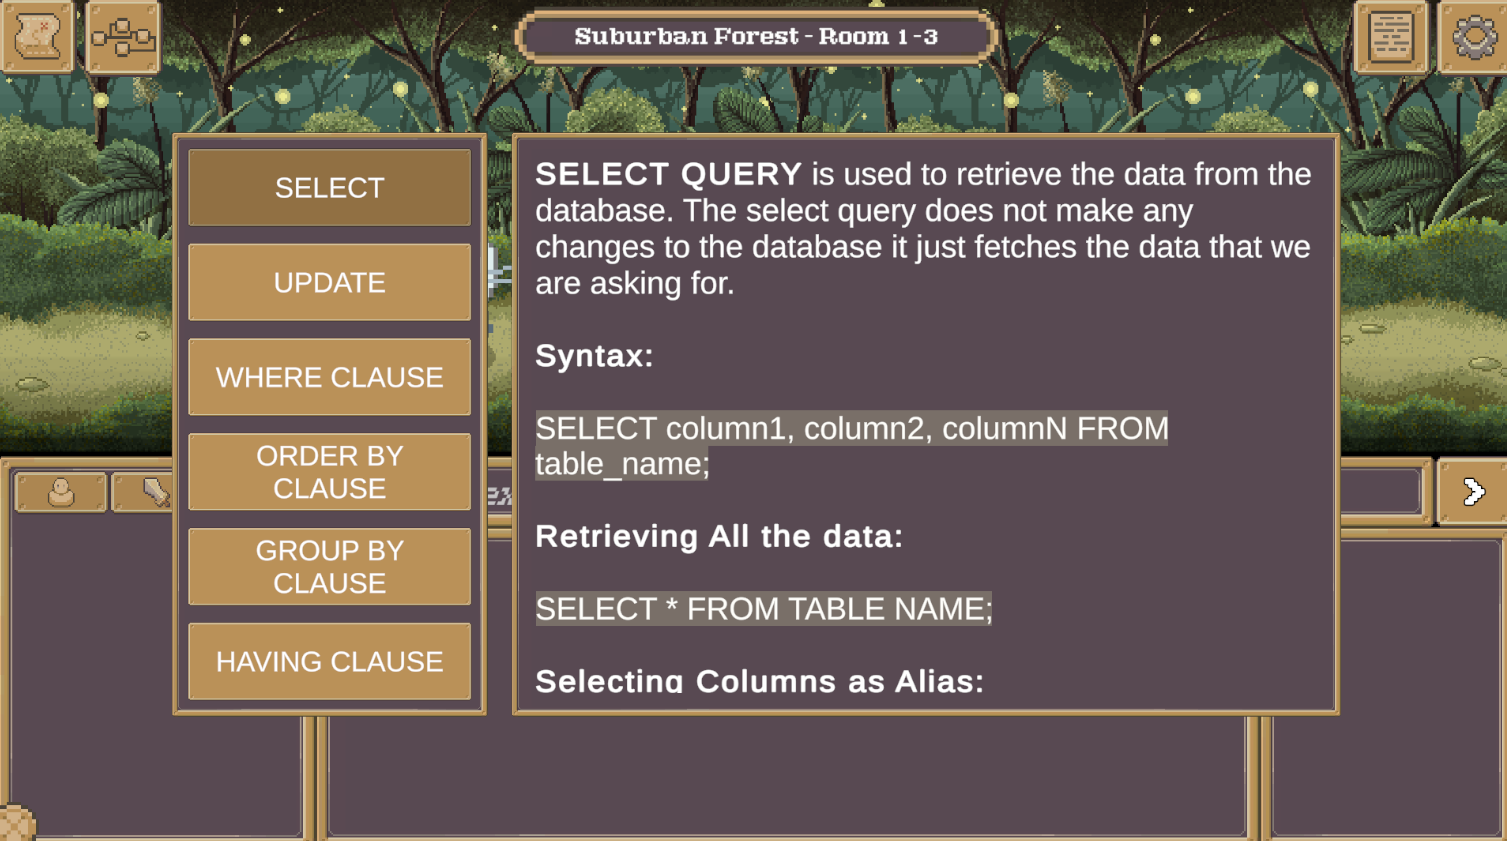
\includegraphics[width=13cm]{Images/DocumentationUI.png}
	\vspace{0.5cm}
	\caption{Minh họa UI tra cứu câu lệnh SQL}
\end{figure}

\subsubsection{Hội hội thoại}

UI hộp hội thoại xuất hiện mỗi khi người chơi đụng độ một quái vật trong màn chơi.

\begin{figure}[H]
	\centering
	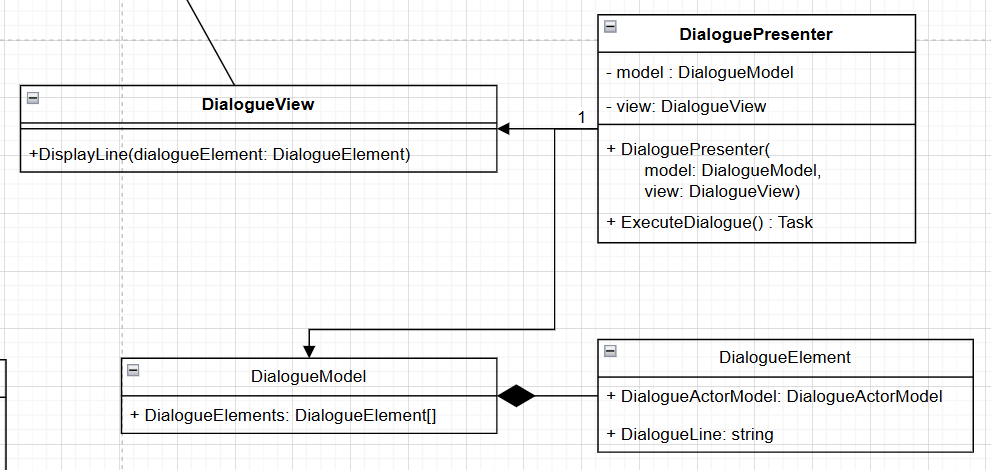
\includegraphics[width=13cm]{Images/DialogueView.png}
	\vspace{0.5cm}
	\caption{Dialogue class diagram}
\end{figure}

\begin{figure}[H]
	\centering
	\includegraphics[width=13cm]{Images/DialogueUI.png}
	\vspace{0.5cm}
	\caption{Minh họa UI đoạn hội thoại}
\end{figure}

\subsubsection{Hiệu ứng pop up text}

Popup text thể hiện sát thương nhận vào hoặc hiệu ứng áp dụng lên người chơi hay quái vật.

\begin{figure}[H]
	\centering
	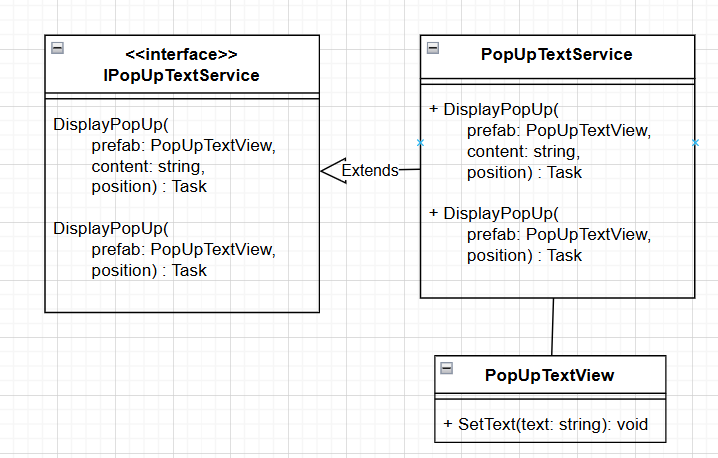
\includegraphics[width=13cm]{Images/PopUpText.png}
	\vspace{0.5cm}
	\caption{Pop up text class diagram}
\end{figure}

\begin{figure}[H]
	\centering
	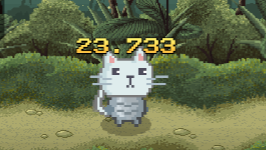
\includegraphics[width=13cm]{Images/PopupTextUI.png}
	\vspace{0.5cm}
	\caption{Minh họa UI Popup text}
\end{figure}

\subsubsection{Hộp thoại thông báo}

Hộp thoại thông báo hệ thống.

\begin{figure}[H]
	\centering
	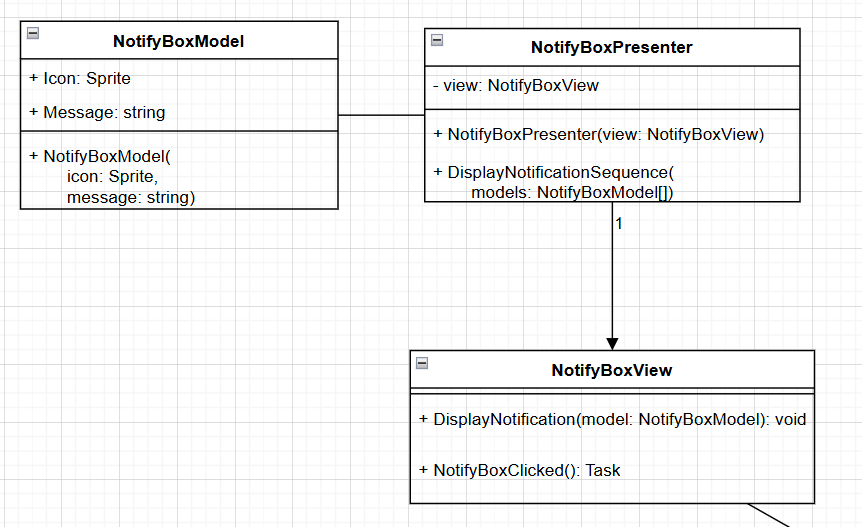
\includegraphics[width=13cm]{Images/NotifyBoxView.png}
	\vspace{0.5cm}
	\caption{Notify box class diagram}
\end{figure}

\begin{figure}[H]
	\centering
	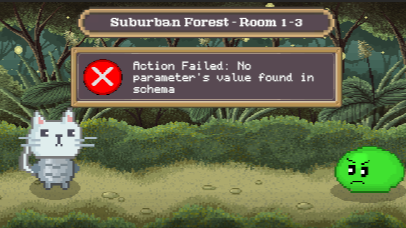
\includegraphics[width=13cm]{Images/NotifyBoxUI.png}
	\vspace{0.5cm}
	\caption{Minh họa UI hộp thoại thông báo}
\end{figure}

\subsubsection{UI cấu trúc màn chơi}

Mỗi màn chơi là một mê cung, người chơi chỉ biết xuất phát điểm và căn phòng đích đến. Để đến được điểm đích, người chơi phải di chuyển qua nhiều căn phòng khác nhau và những căn phòng này chỉ được lộ diện khi người chơi đã chinh phục căn phòng hiện tại.

\begin{figure}[H]
	\centering
	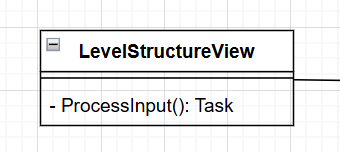
\includegraphics[width=7cm]{Images/LevelStructureView.png}
	\vspace{0.5cm}
	\caption{Level structure view}
\end{figure}

\begin{figure}[H]
	\centering
	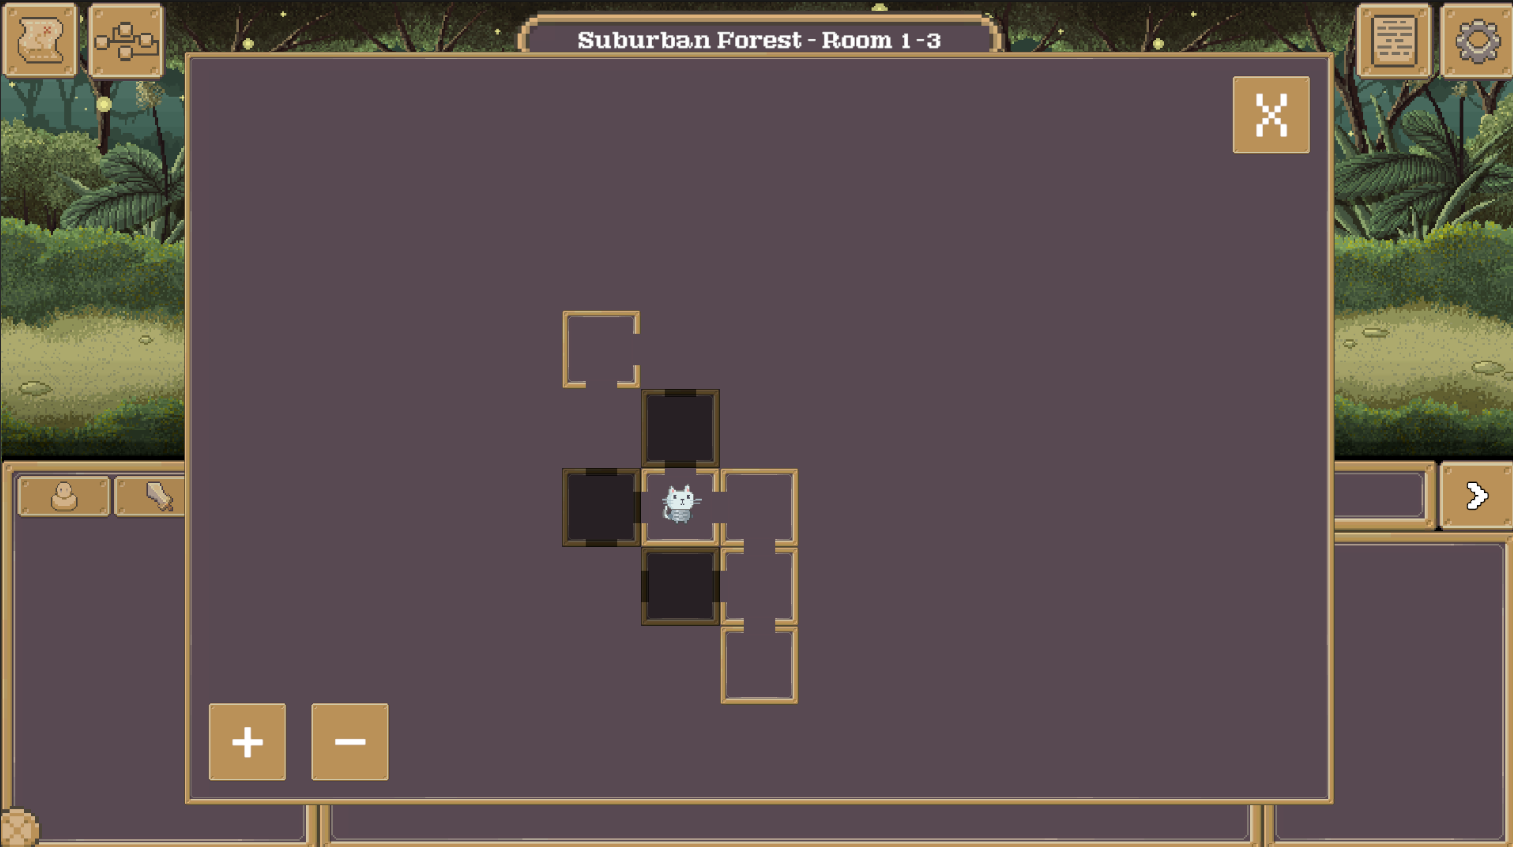
\includegraphics[width=13cm]{Images/LevelStructureUI.png}
	\vspace{0.5cm}
	\caption{Minh họa UI cấu trúc màn chơi}
\end{figure}

Để mô phỏng được cấu trúc mê cung của một màn chơi thì nhóm nghiên cứu sử dụng cấu trúc dữ liệu là đồ thị.

\begin{figure}[H]
	\centering
	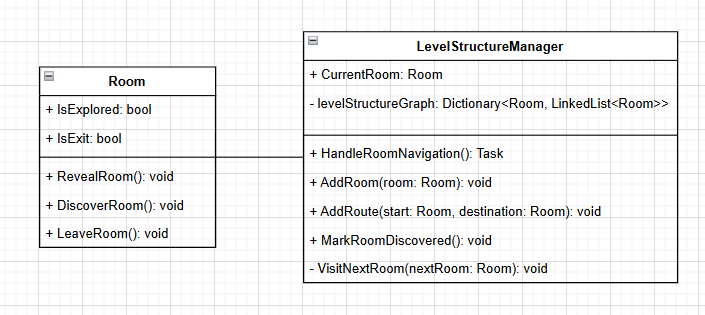
\includegraphics[width=13cm]{Images/LevelStructureManager.png}
	\vspace{0.5cm}
	\caption{Level strucutre class diagram}
\end{figure}